\section{Imagenes de los ensayos}

    % ========== BANCO DE PRUEBA ==========
\begin{center}
    \centering
    \includegraphics[width=0.9\linewidth]{./imagenes/banco_prueba_frente.jpg}
    \captionof{figure}{Banco de pruebas utilizado en las mediciones.}
\end{center}

\begin{center}
    \centering
    \includegraphics[width=0.9\linewidth]{./imagenes/fuente_completa.jpg}
    \captionof{figure}{Fuente de alimentación ensamblada completamente.}
\end{center}

\begin{center}
    \centering
    \includegraphics[width=0.9\linewidth]{./imagenes/fuente_sin_LM317.jpg}
    \captionof{figure}{Fuente sin el integrado LM317.}
\end{center}

\begin{center}
    \centering
    \includegraphics[width=0.9\linewidth]{./imagenes/reostato.jpg}
    \captionof{figure}{Reóstato utilizado en las pruebas.}
\end{center}

\saltoPag{}

% ========== PLACA ==========
\begin{center}
    \centering
    \includegraphics[width=0.9\linewidth]{./imagenes/placa_completa.jpg}
    \captionof{figure}{Placa de circuito impreso terminada.}
\end{center}

% ========== TENSIONES BAJAS ==========

\begin{center}
    \centering
    \includegraphics[width=0.9\linewidth]{./imagenes/tension_baja_vacio.jpg}
    \captionof{figure}{Tensión baja en vacío.}
\end{center}


\begin{center}
    \centering
    \includegraphics[width=0.9\linewidth]{./imagenes/tension_baja_050.jpg}
    \captionof{figure}{Medición de tensión baja (0.50 V).}
\end{center}

\begin{center}
    \centering
    \includegraphics[width=0.9\linewidth]{./imagenes/tension_baja_075.jpg}
    \captionof{figure}{Medición de tensión baja (0.75 V).}
\end{center}

\begin{center}
    \centering
    \includegraphics[width=0.9\linewidth]{./imagenes/tension_baja_1,25.jpg}
    \captionof{figure}{Medición de tensión baja (1.25 V).}
\end{center}

\begin{center}
    \centering
    \includegraphics[width=0.9\linewidth]{./imagenes/tension_baja_1,50.jpg}
    \captionof{figure}{Medición de tensión baja (1.50 V).}
\end{center}


% ========== CORRIENTES BAJAS ==========
\begin{center}
    \centering
    \includegraphics[width=0.9\linewidth]{./imagenes/corriente_baja_0,25.jpg}
    \captionof{figure}{Medición de corriente baja (0.25 A).}
\end{center}

\begin{center}
    \centering
    \includegraphics[width=0.9\linewidth]{./imagenes/corriente_baja_050.jpg}
    \captionof{figure}{Medición de corriente baja (0.50 A).}
\end{center}

\begin{center}
    \centering
    \includegraphics[width=0.9\linewidth]{./imagenes/corriente_baja_075.jpg}
    \captionof{figure}{Medición de corriente baja (0.75 A).}
\end{center}

\saltoPag{}

\begin{center}
    \centering
    \includegraphics[width=0.9\linewidth]{./imagenes/corriente_baja_1,25.jpg}
    \captionof{figure}{Medición de corriente baja (1.25 A).}
\end{center}

\begin{center}
    \centering
    \includegraphics[width=0.9\linewidth]{./imagenes/corriente_baja_1,5.jpg}
    \captionof{figure}{Medición de corriente baja (1.5 A).}
\end{center}

% ========== RIPPLE BAJO ==========
\begin{center}
    \centering
    \includegraphics[width=0.9\linewidth]{./imagenes/riplle_baja_osc_mult.jpg}
    \captionof{figure}{Medición de ripple en baja tensión (osciloscopio y multímetro).}
\end{center}

% ========== TENSIONES ALTAS ==========

\begin{center}
    \centering
    \includegraphics[width=0.9\linewidth]{./imagenes/tension_alta_vacio_rao.jpg}
    \captionof{figure}{Tensión alta en vacío.}
\end{center}


\begin{center}
    \centering
    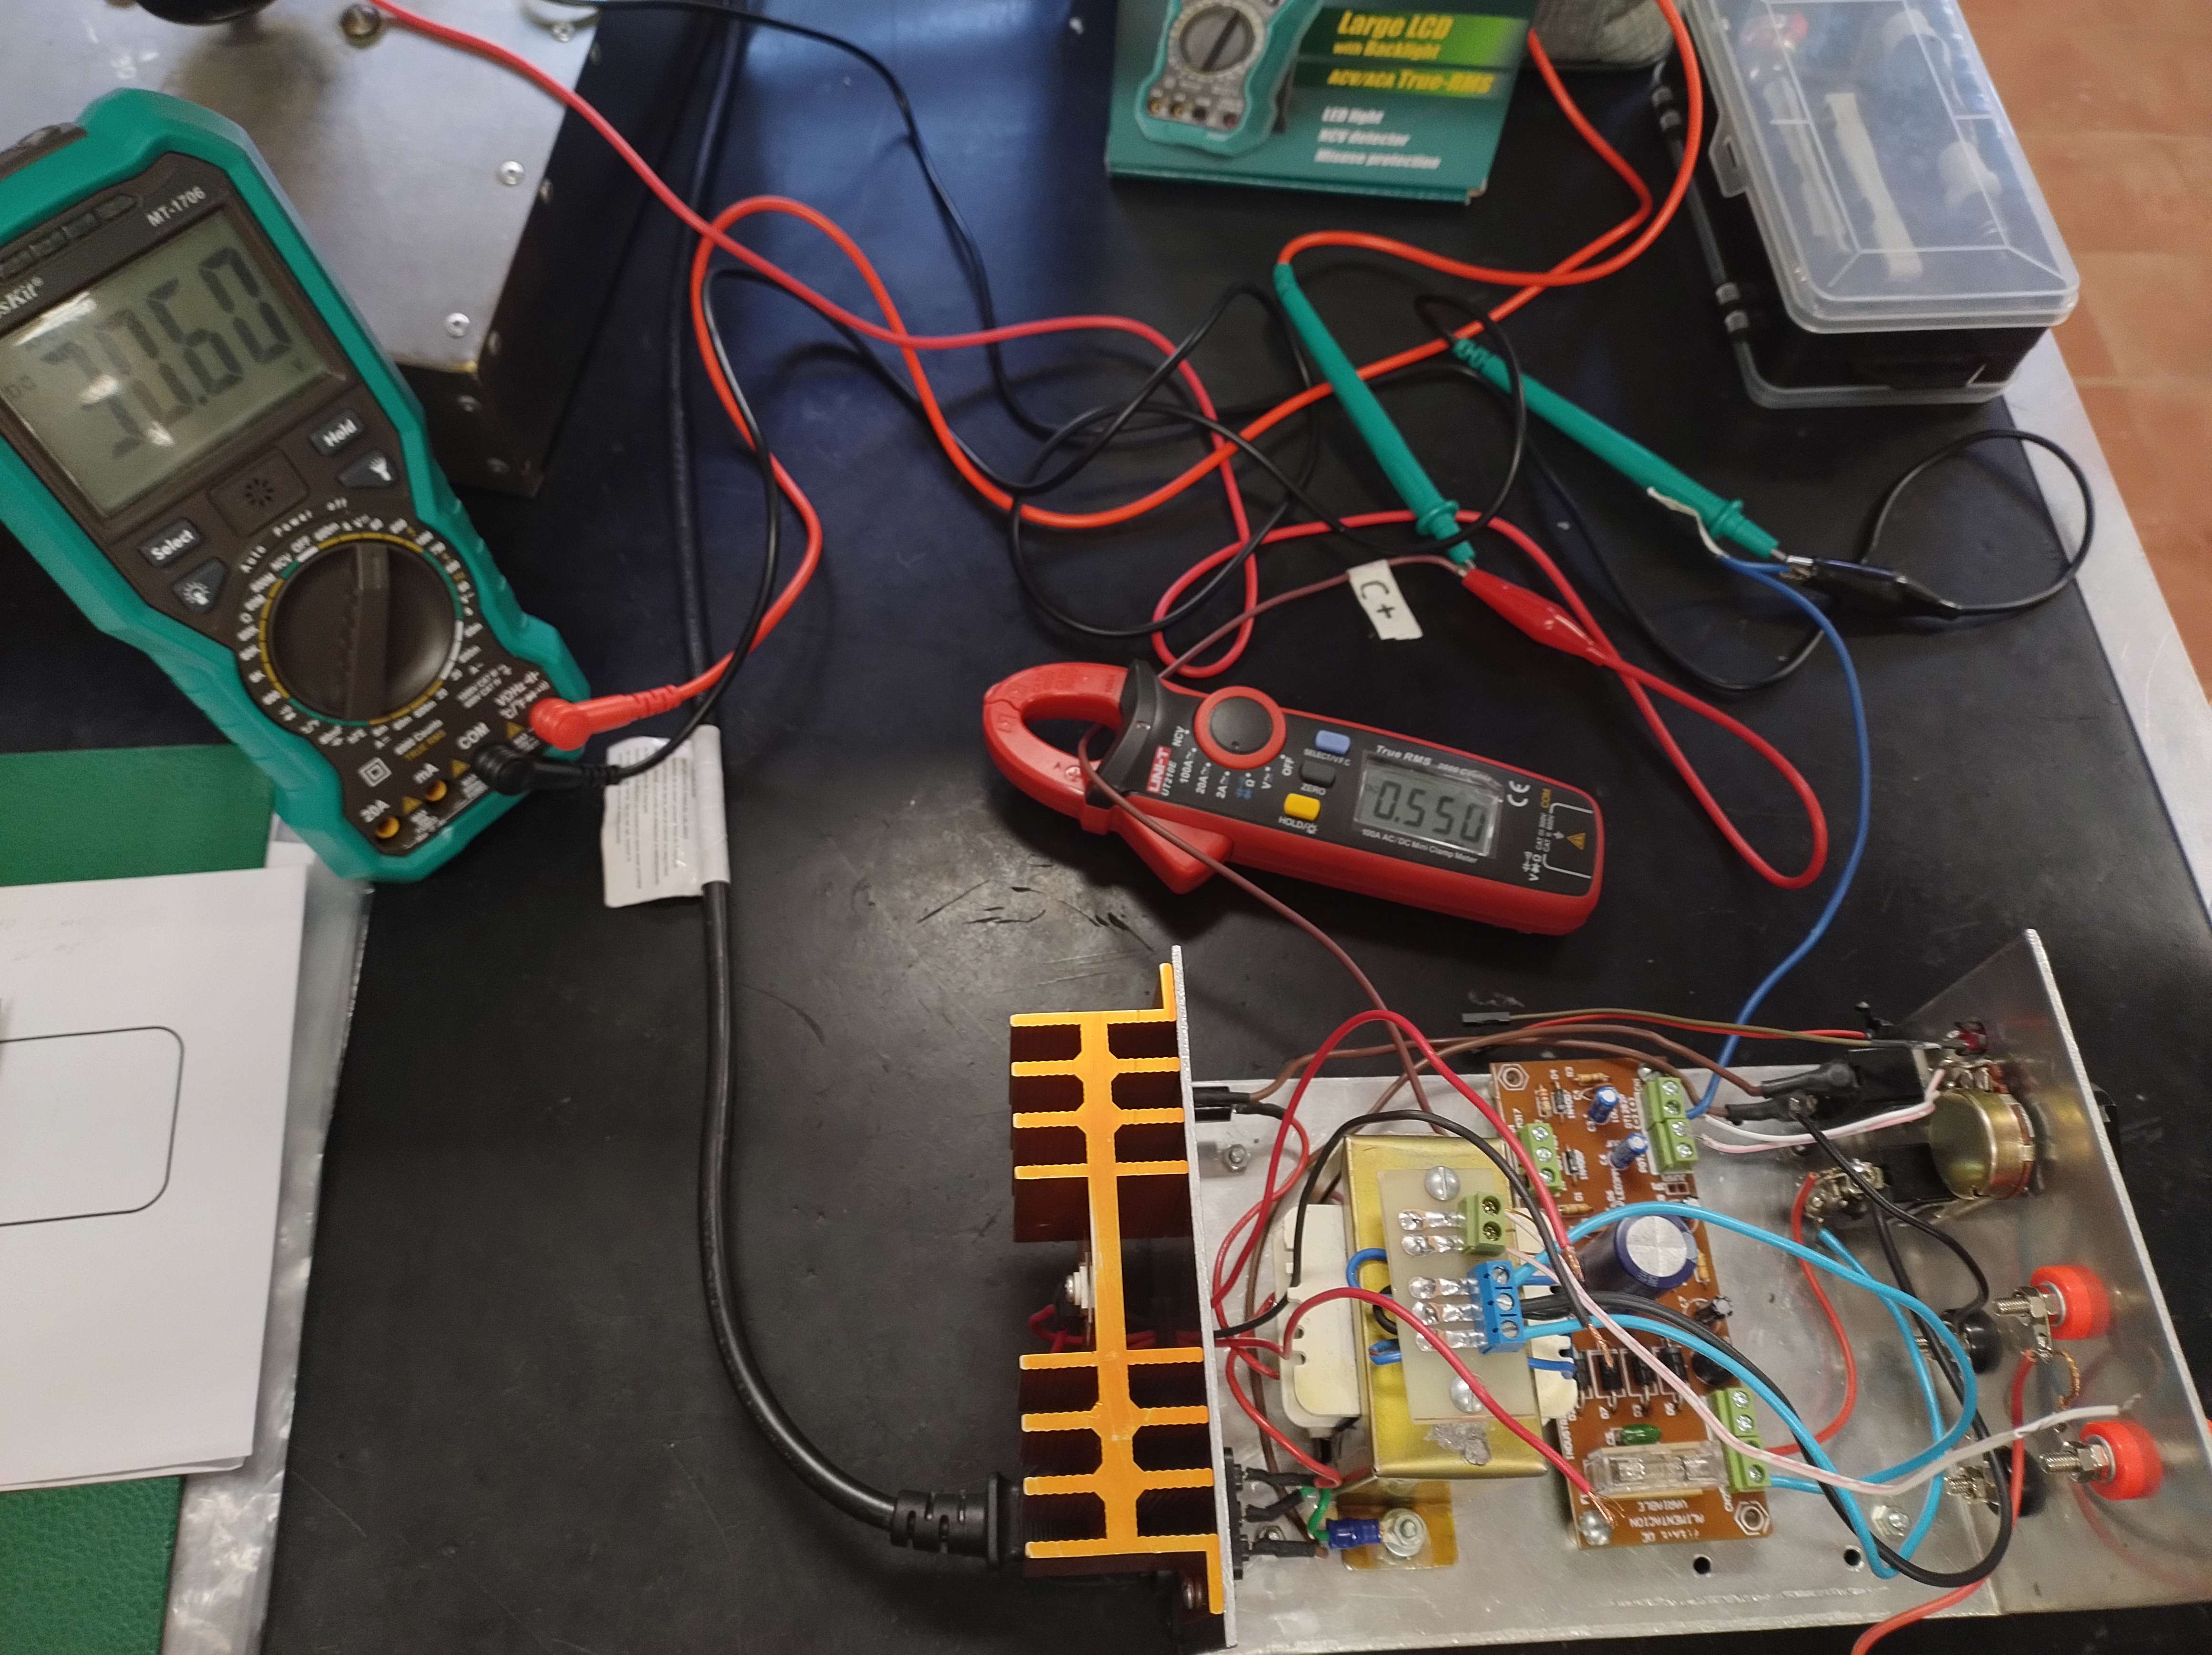
\includegraphics[width=0.9\linewidth]{./imagenes/tension_alta_0,50.jpg}
    \captionof{figure}{Medición de tensión alta (0.50 V).}
\end{center}

\saltoPag{}

\begin{center}
    \centering
    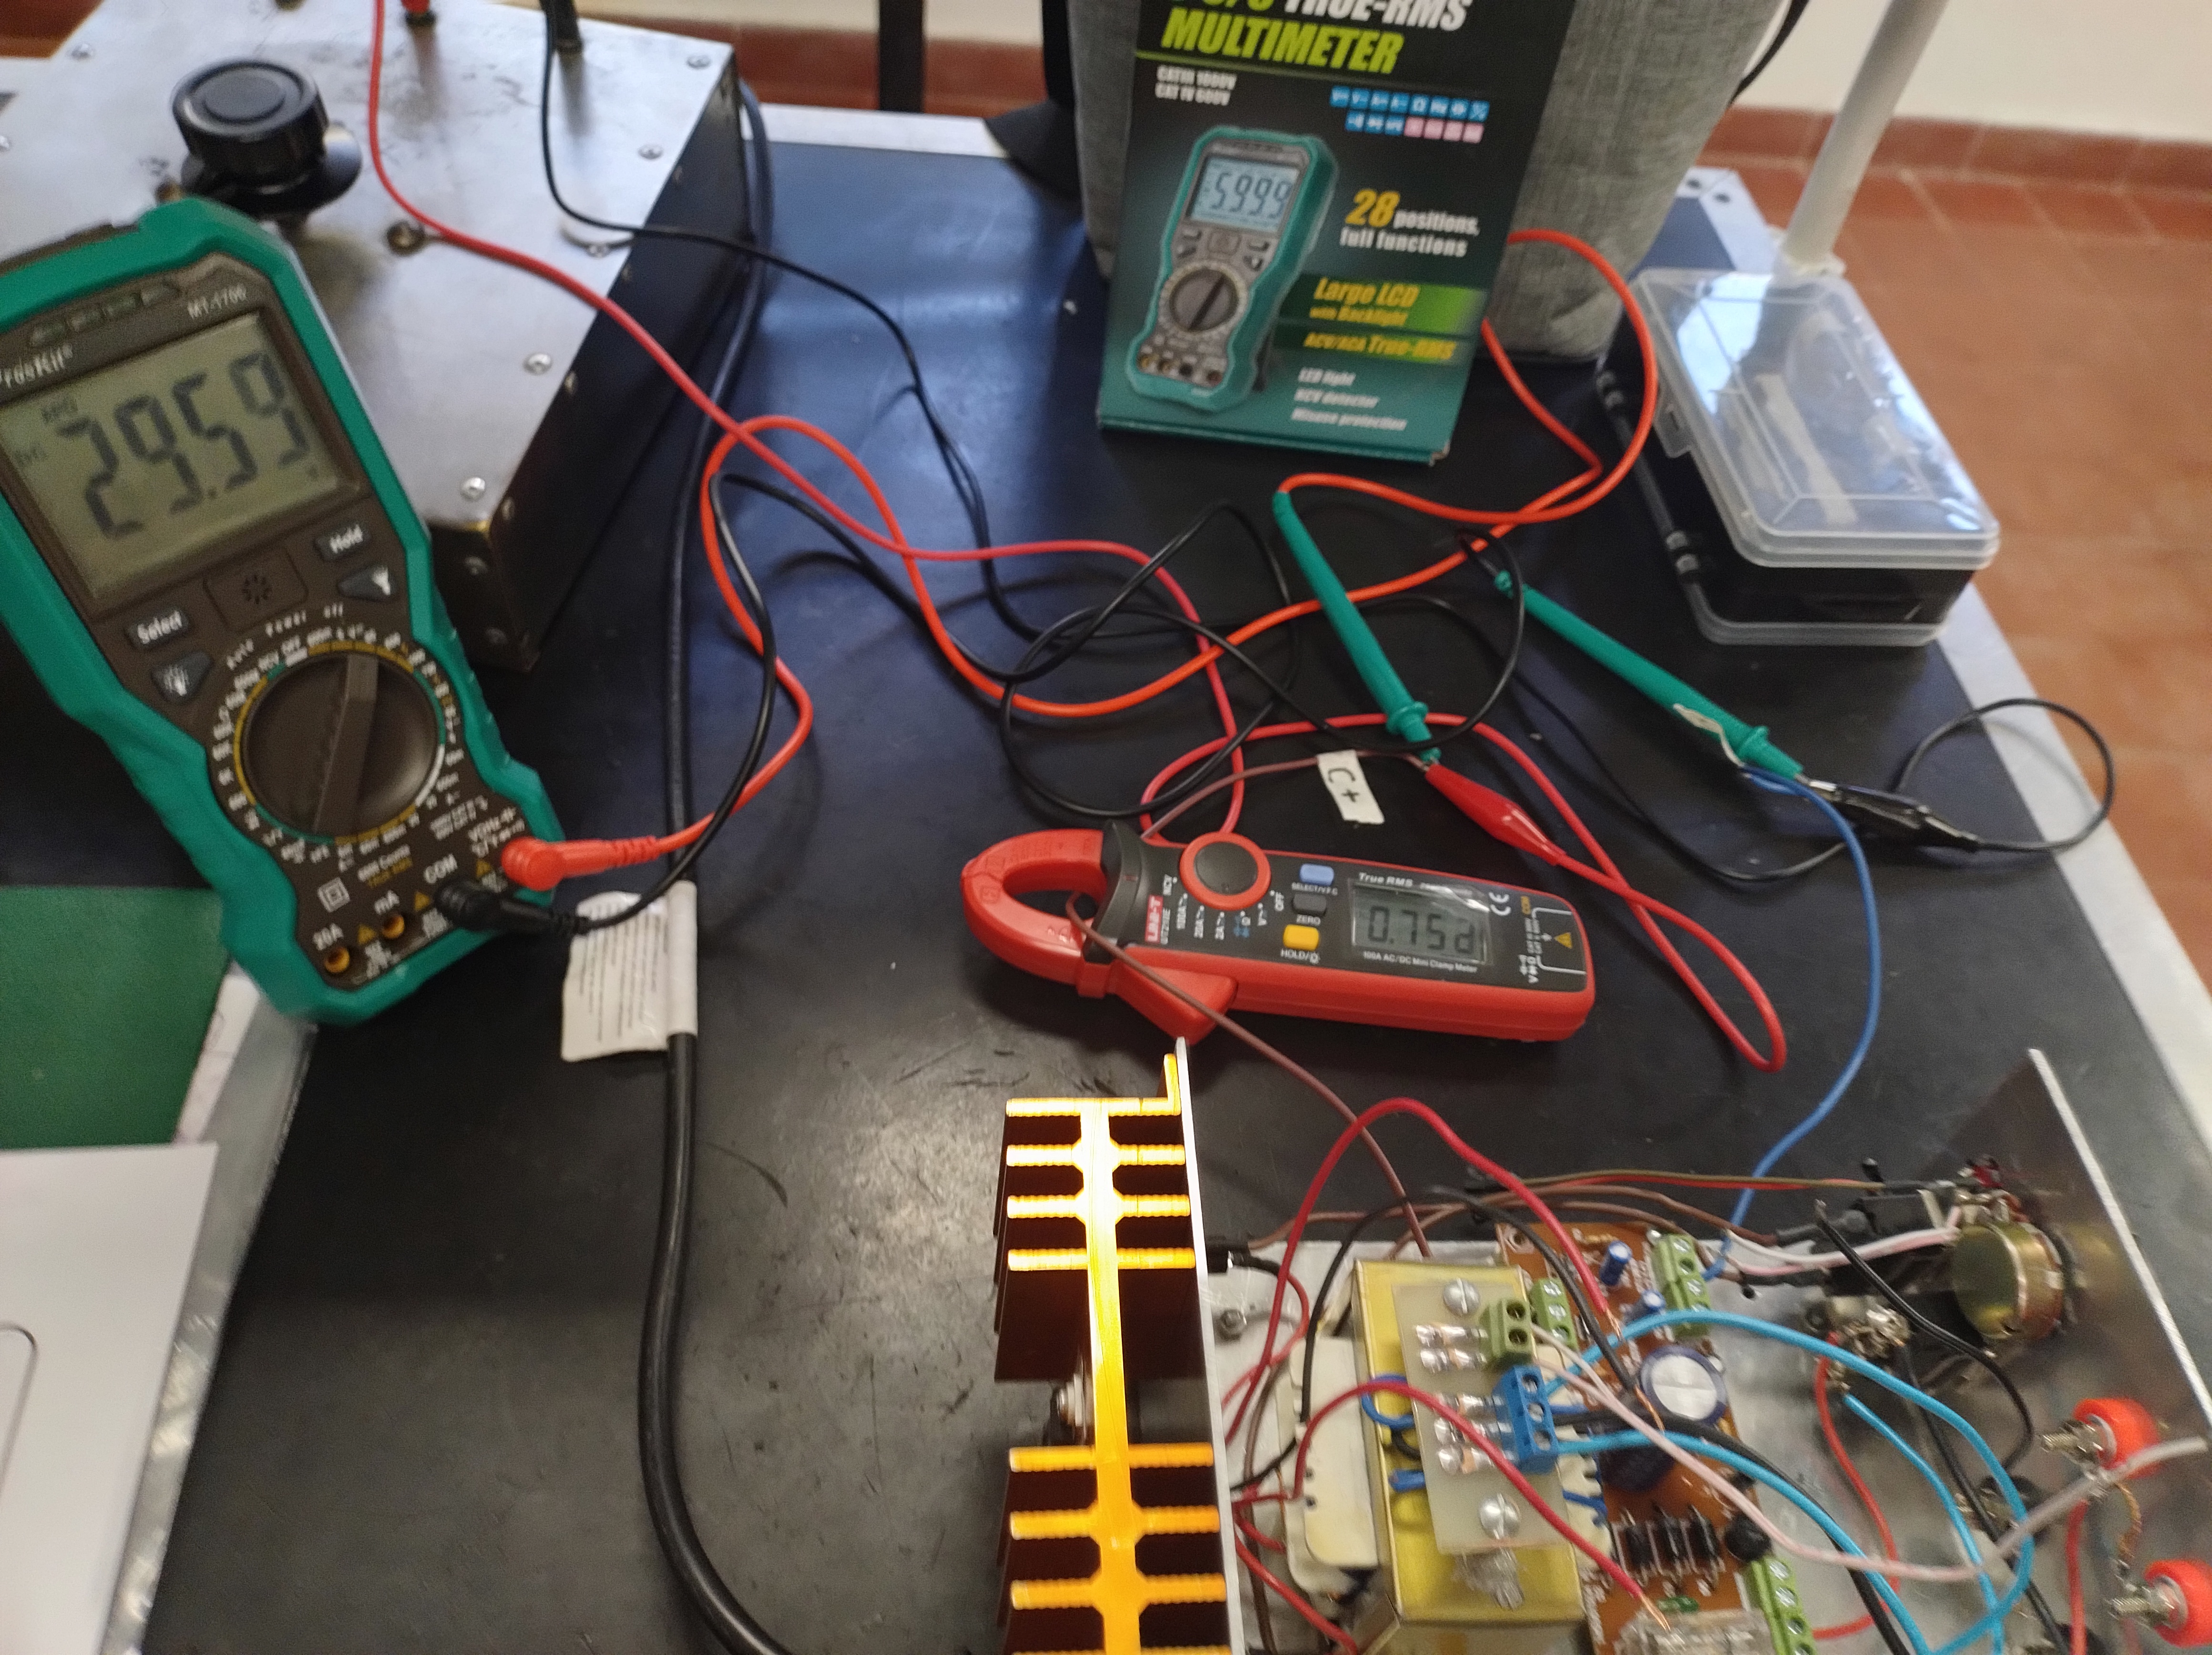
\includegraphics[width=0.9\linewidth]{./imagenes/tension_alta_0,75.jpg}
    \captionof{figure}{Medición de tensión alta (0.75 V).}
\end{center}

\begin{center}
    \centering
    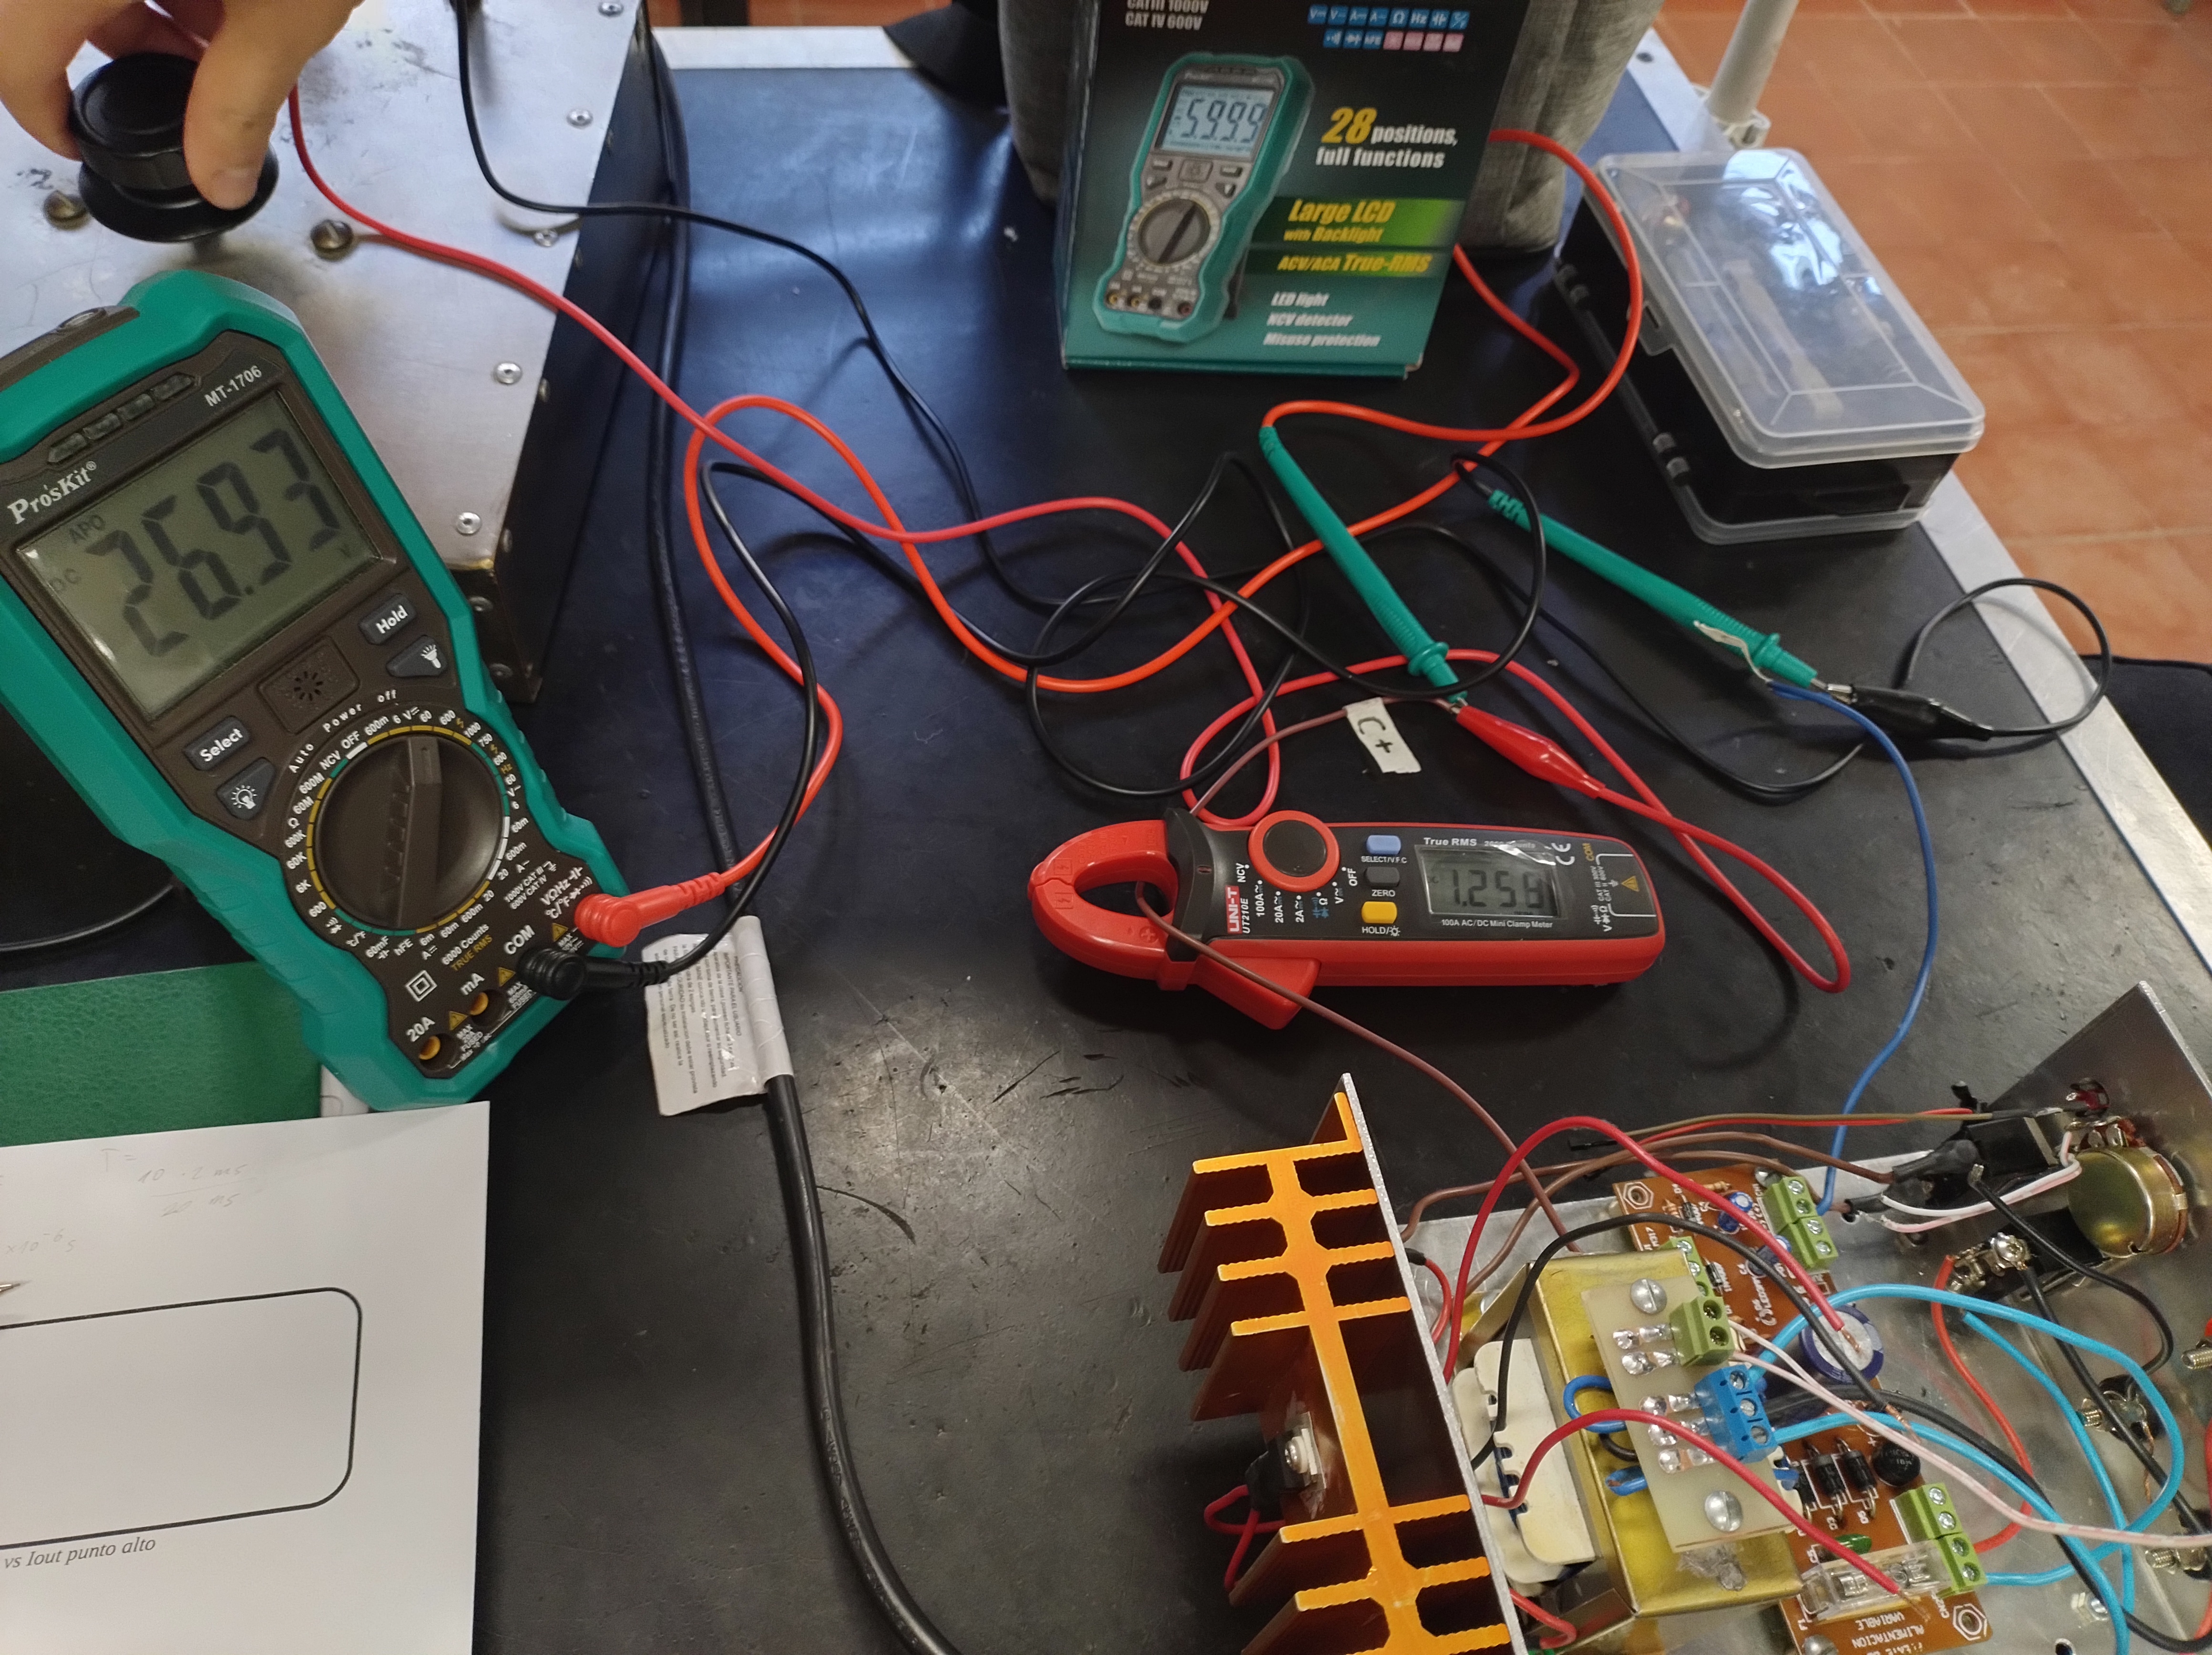
\includegraphics[width=0.9\linewidth]{./imagenes/tension_alta_1,25.jpg}
    \captionof{figure}{Medición de tensión alta (1.25 V).}
\end{center}

\begin{center}
    \centering
    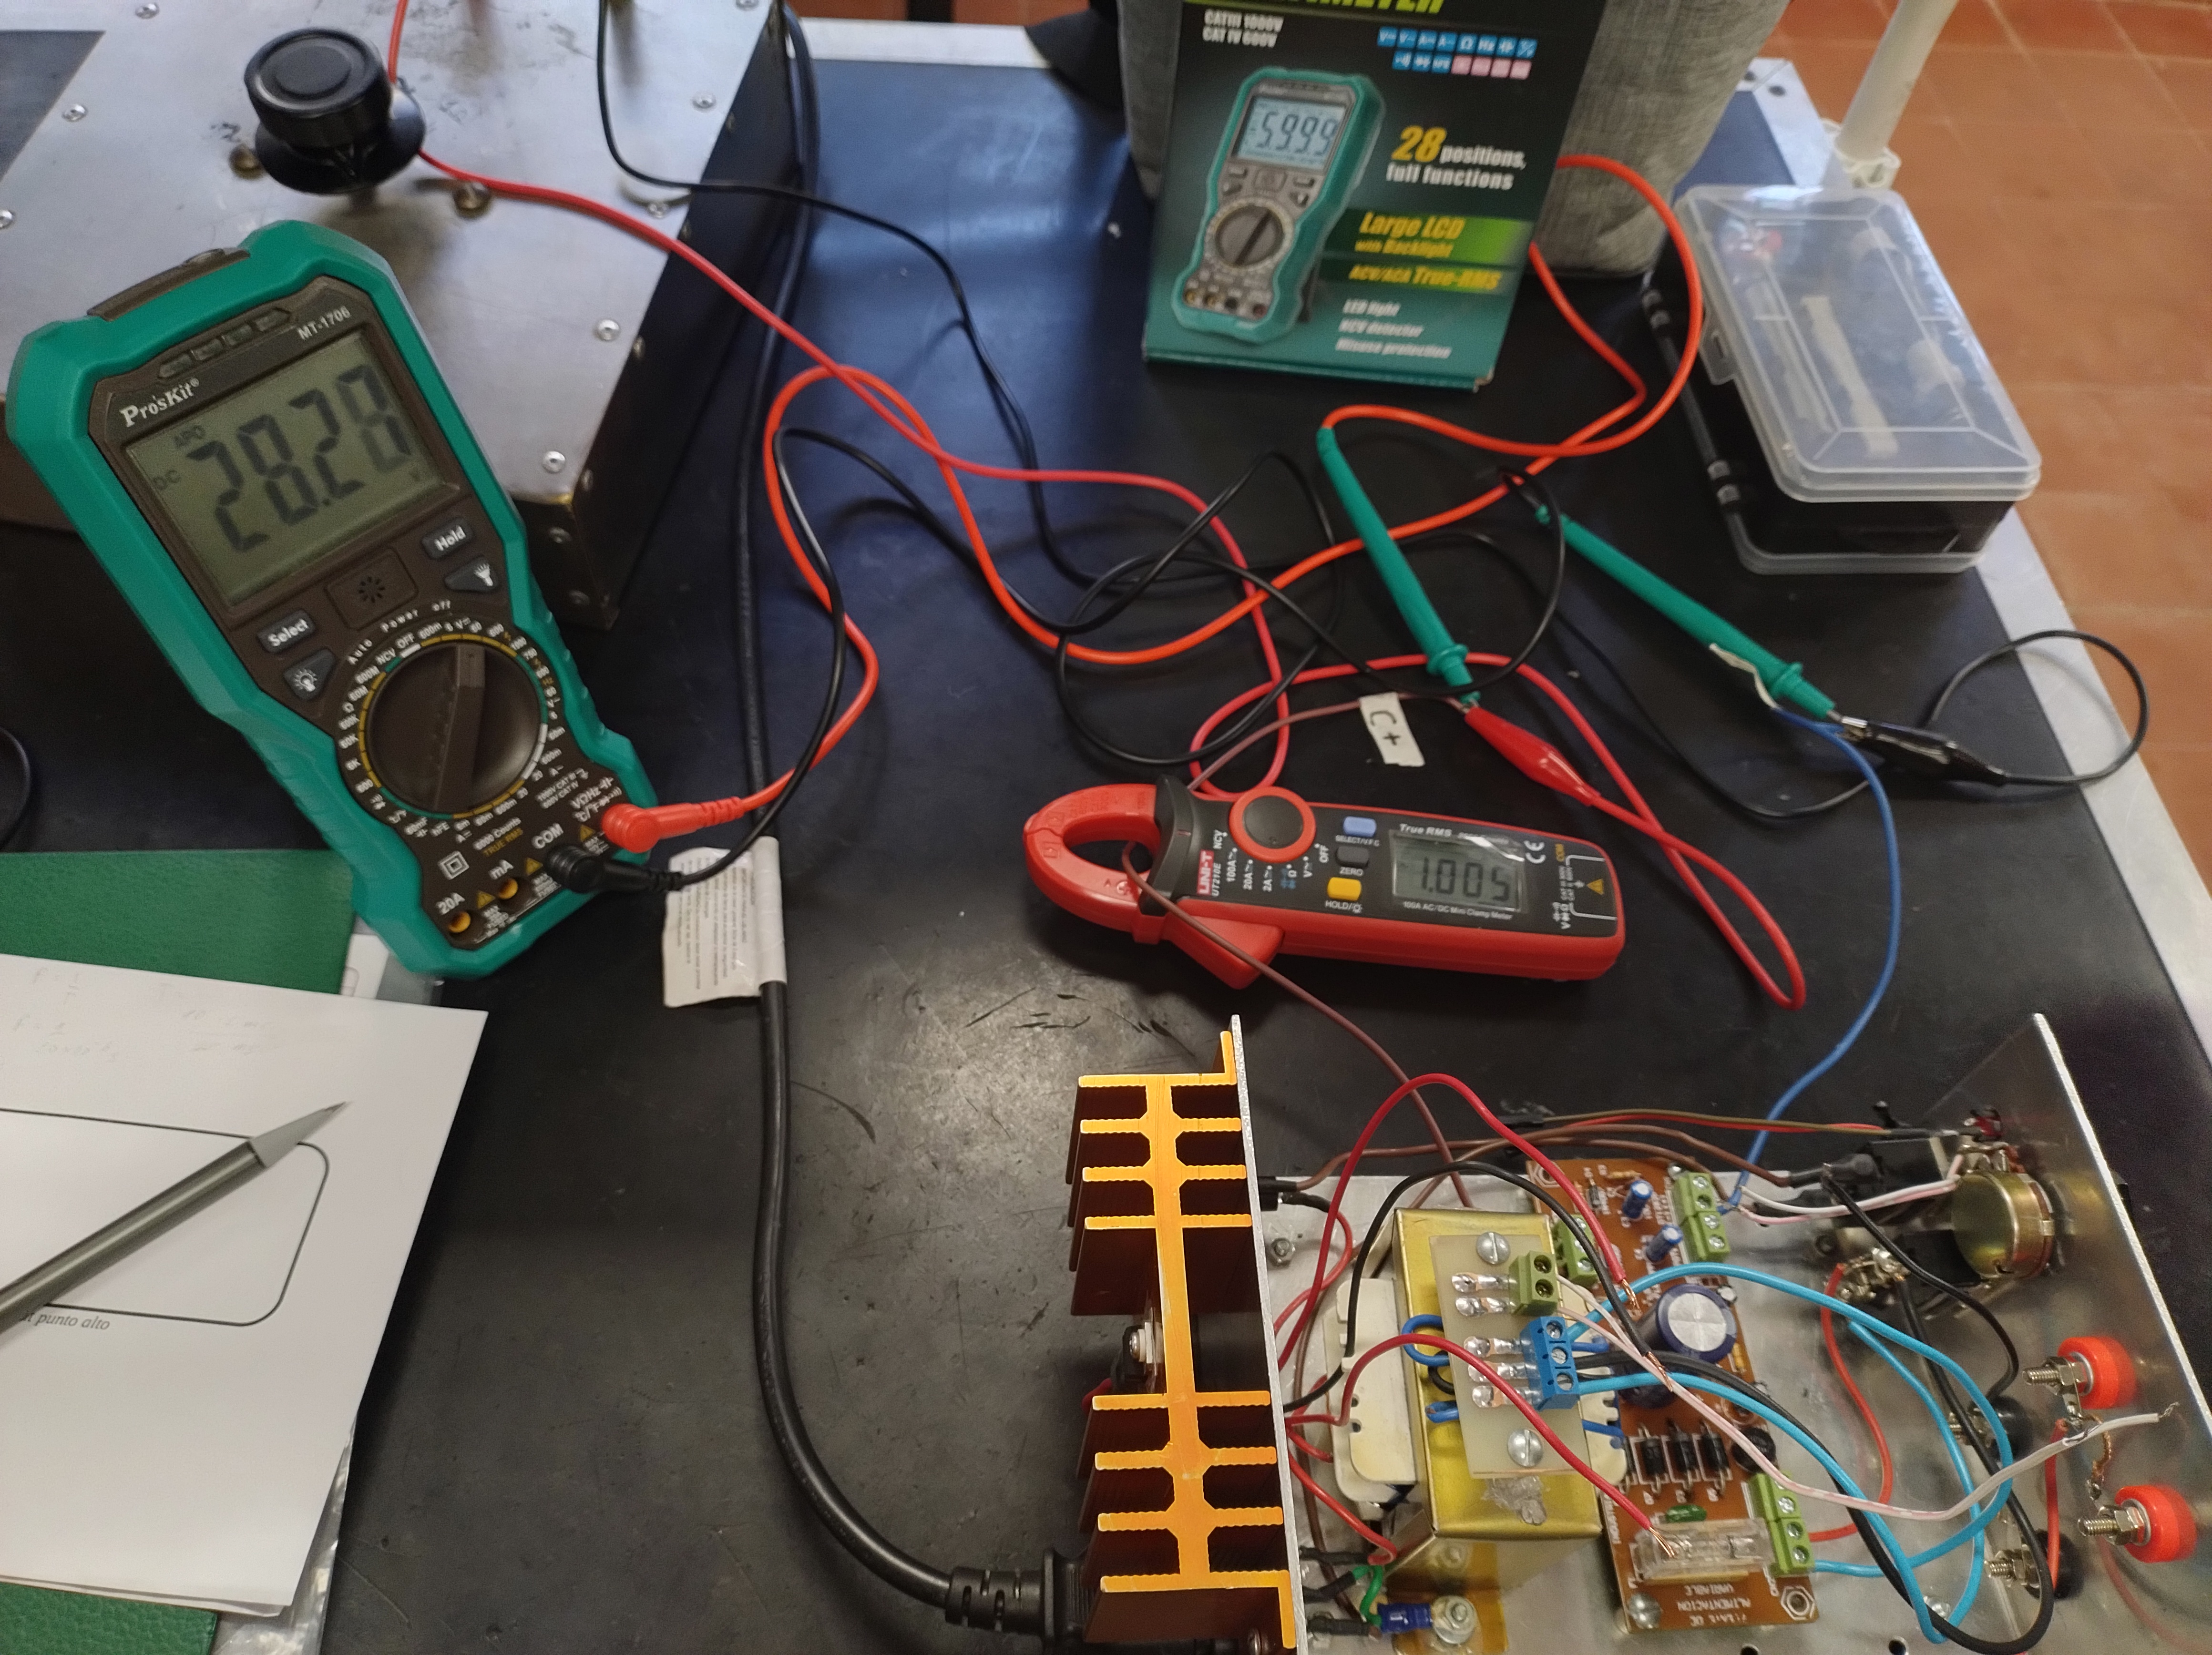
\includegraphics[width=0.9\linewidth]{./imagenes/tension_alta_1.jpg}
    \captionof{figure}{Medición de tensión alta (1 V).}
\end{center}

\vspace{-0.4cm}

\begin{center}
    \centering
    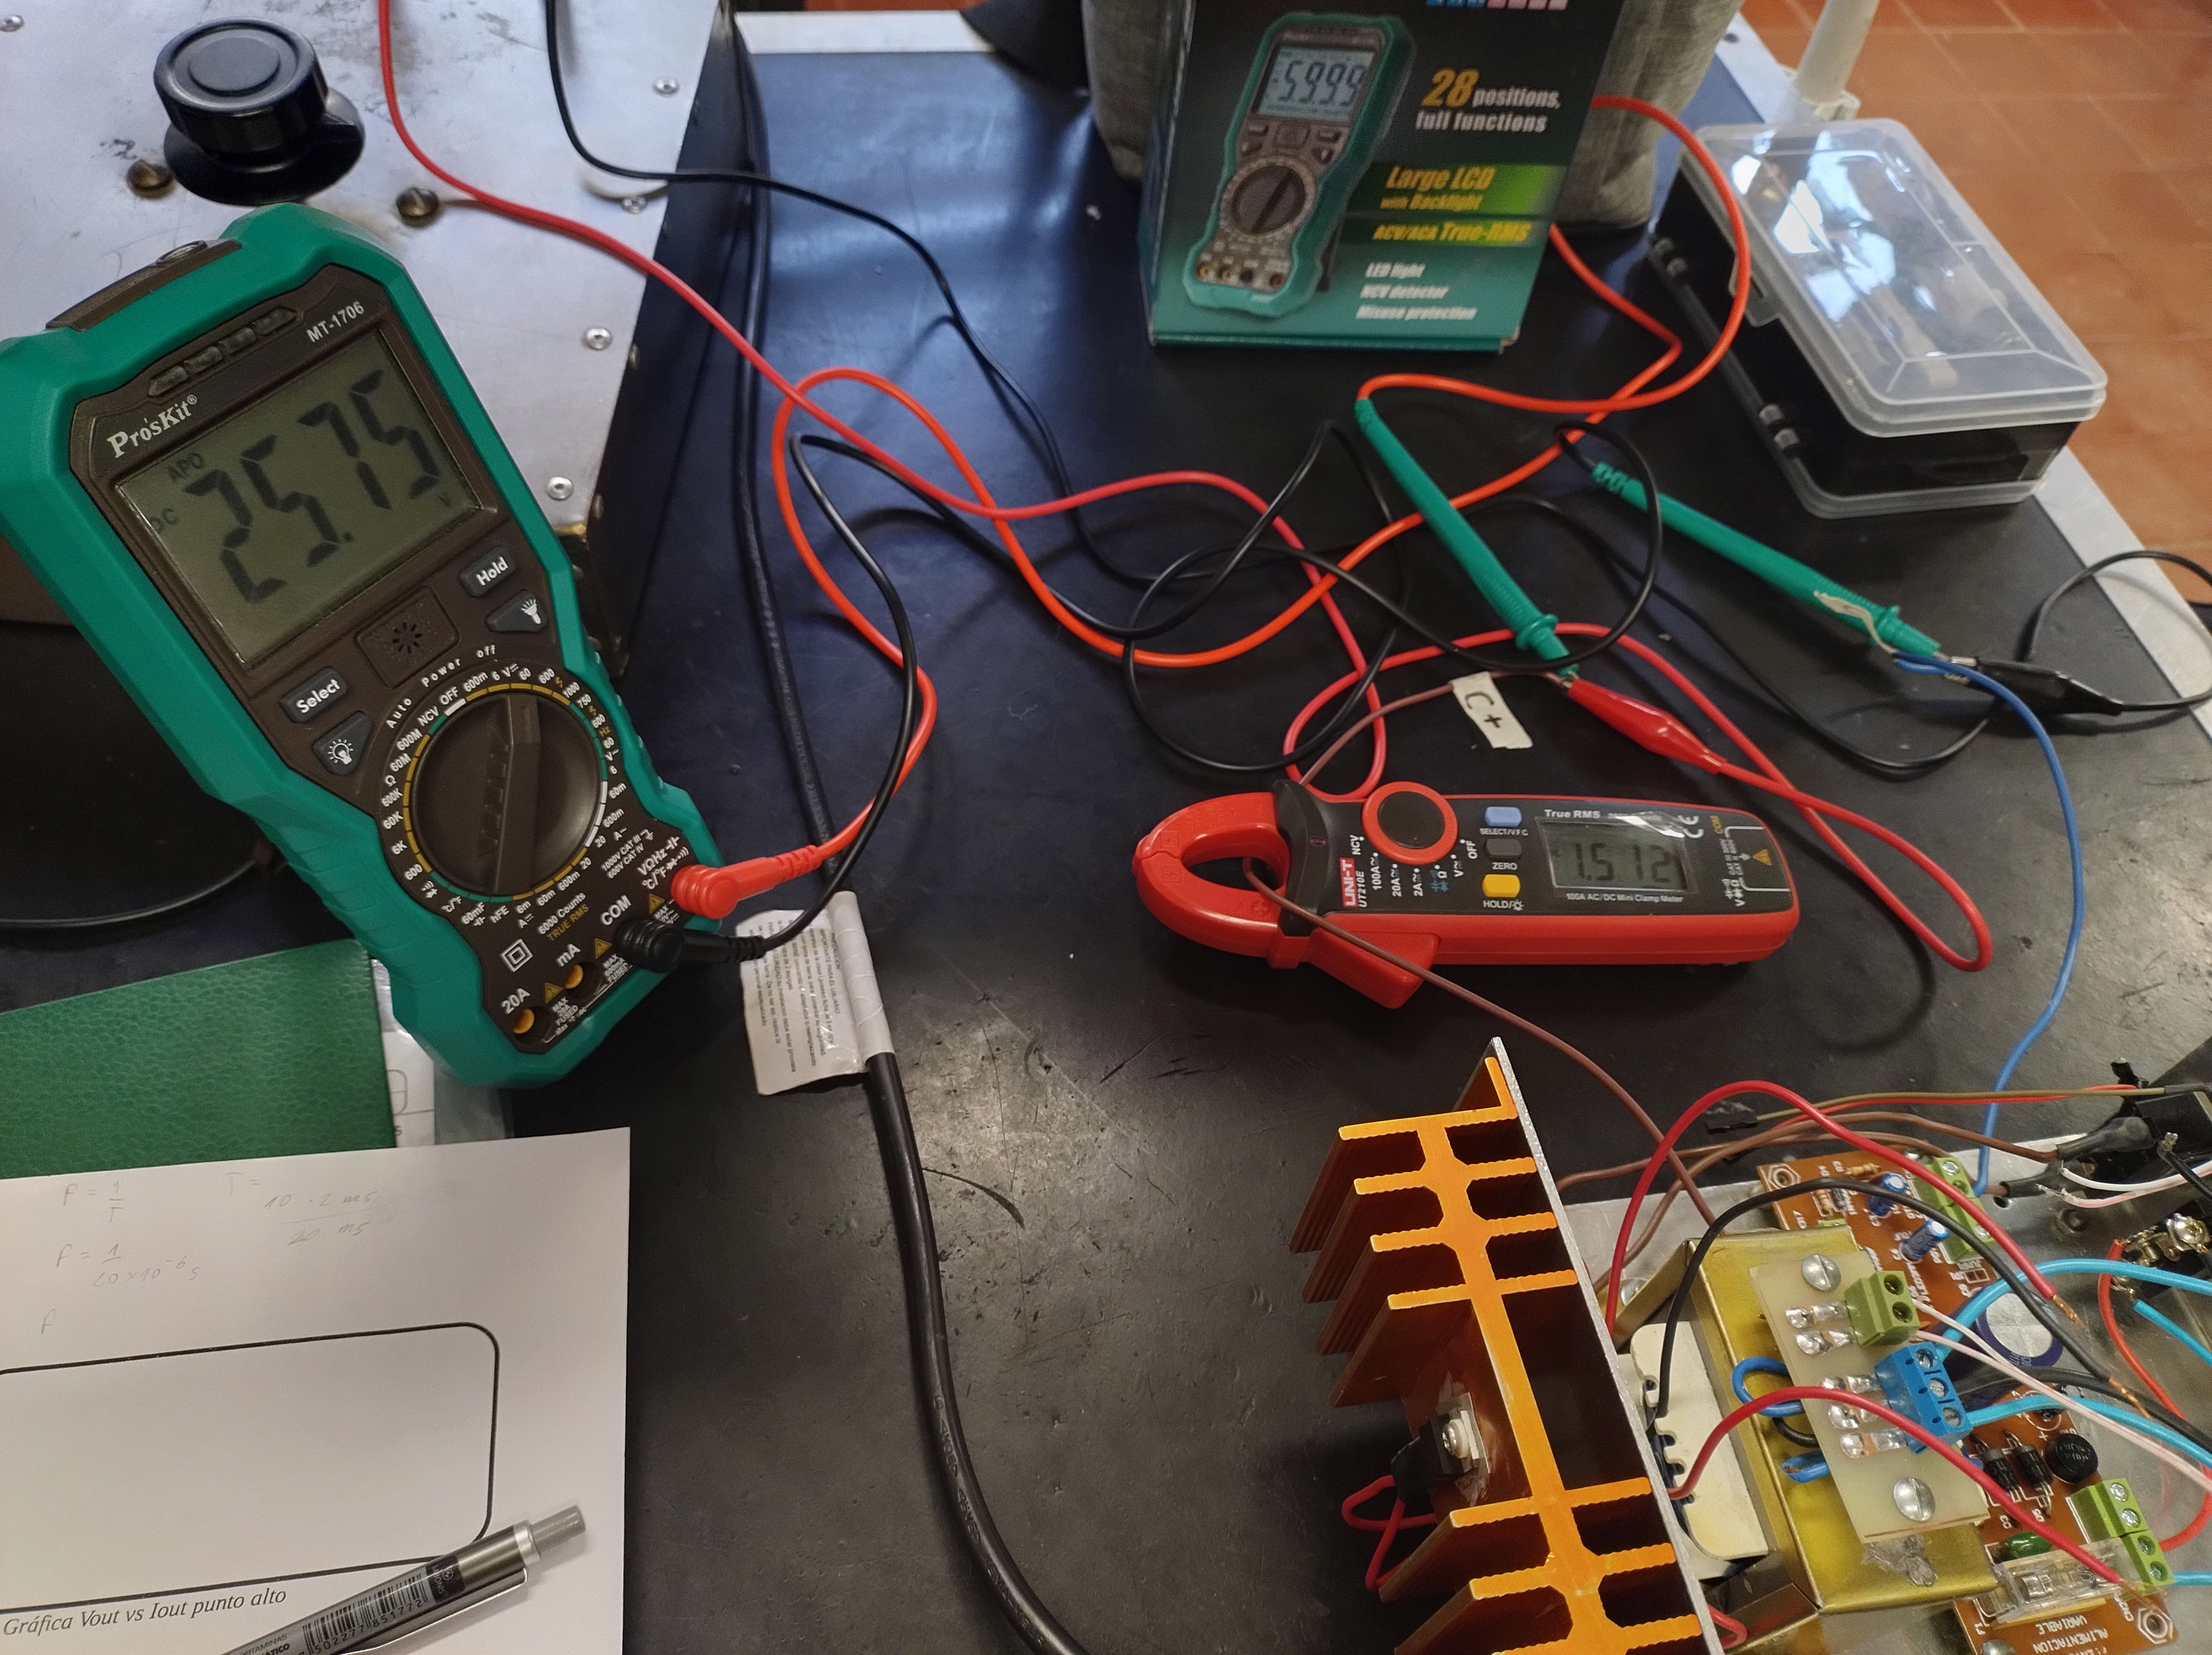
\includegraphics[width=0.9\linewidth]{./imagenes/tension_alta_1,5.jpg}
    \captionof{figure}{Medición de tensión alta (1.5 V).}
\end{center}

\begin{center}
    \centering
    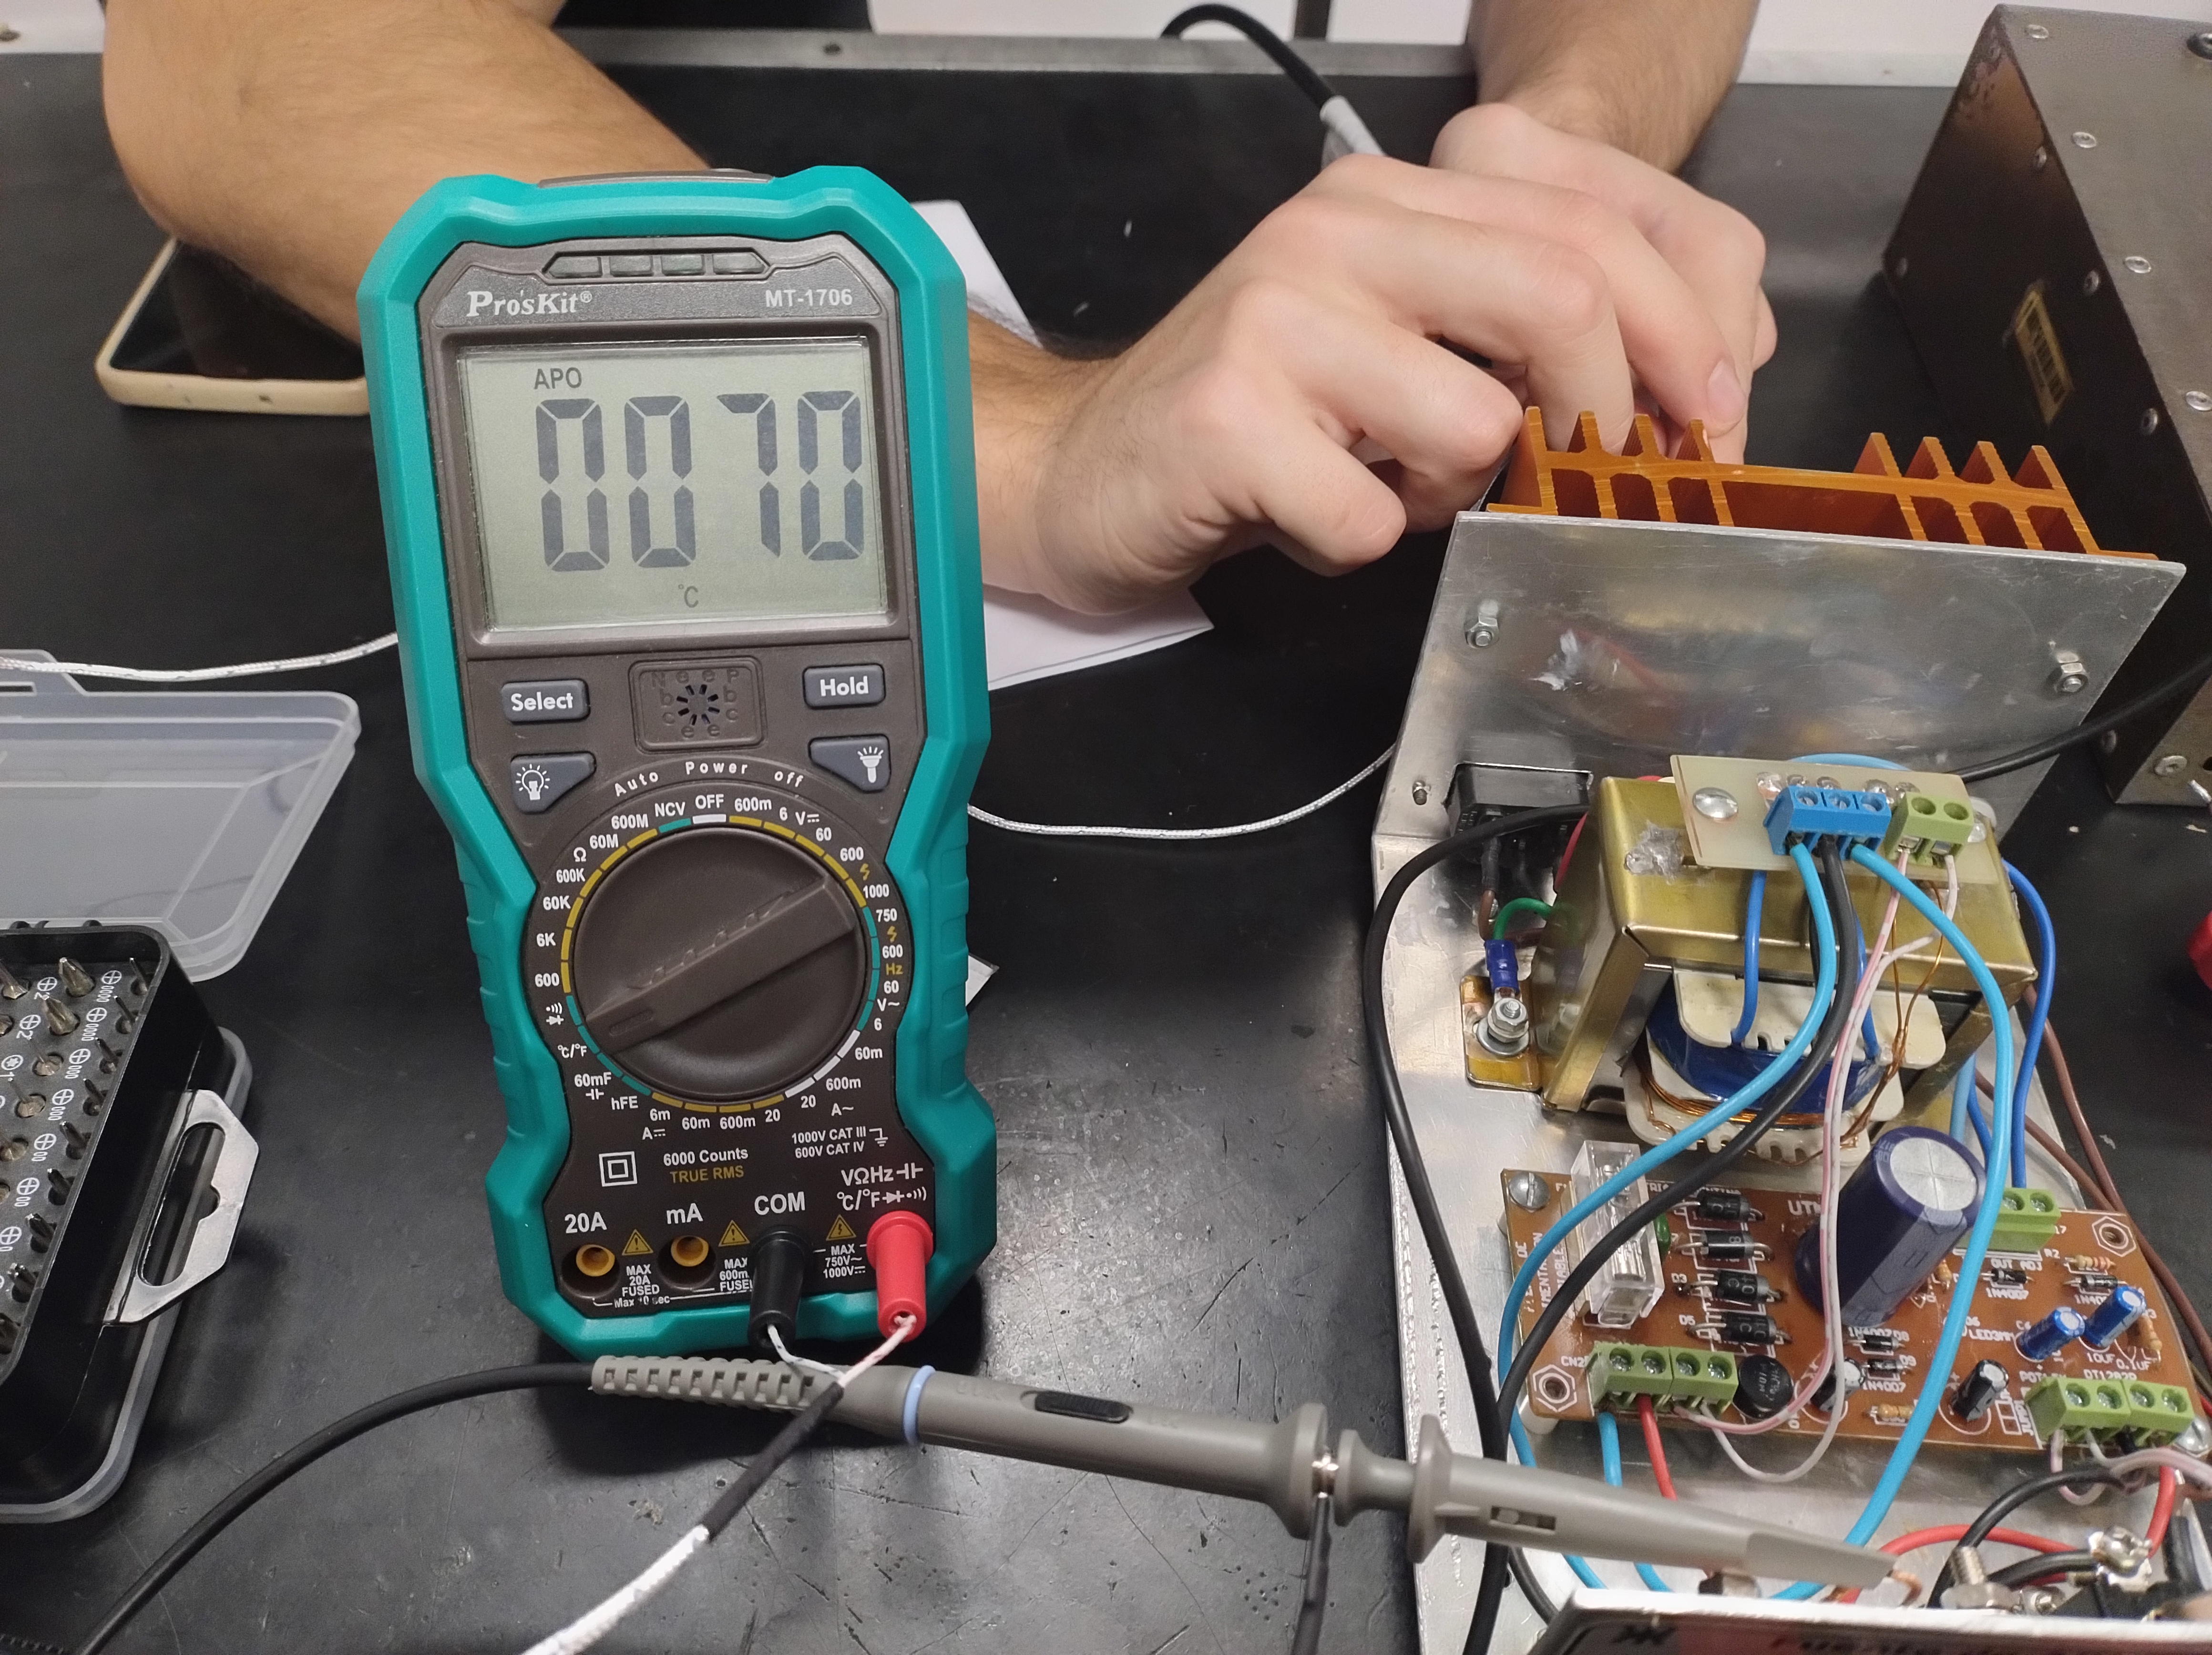
\includegraphics[width=0.9\linewidth]{./imagenes/temperatura_capsula.jpg}
    \captionof{figure}{Temperatura en la cápsula del componente.}
\end{center}


% ========== CORRIENTES ALTAS ==========
\begin{center}
    \centering
    \includegraphics[width=0.9\linewidth]{./imagenes/tension_corriente_alta_vacio.jpg}
    \captionof{figure}{Medición de corriente alta en vacío.}
\end{center}

\saltoPag{}

% ========== RIPPLE ALTO ==========
\begin{center}
    \centering
    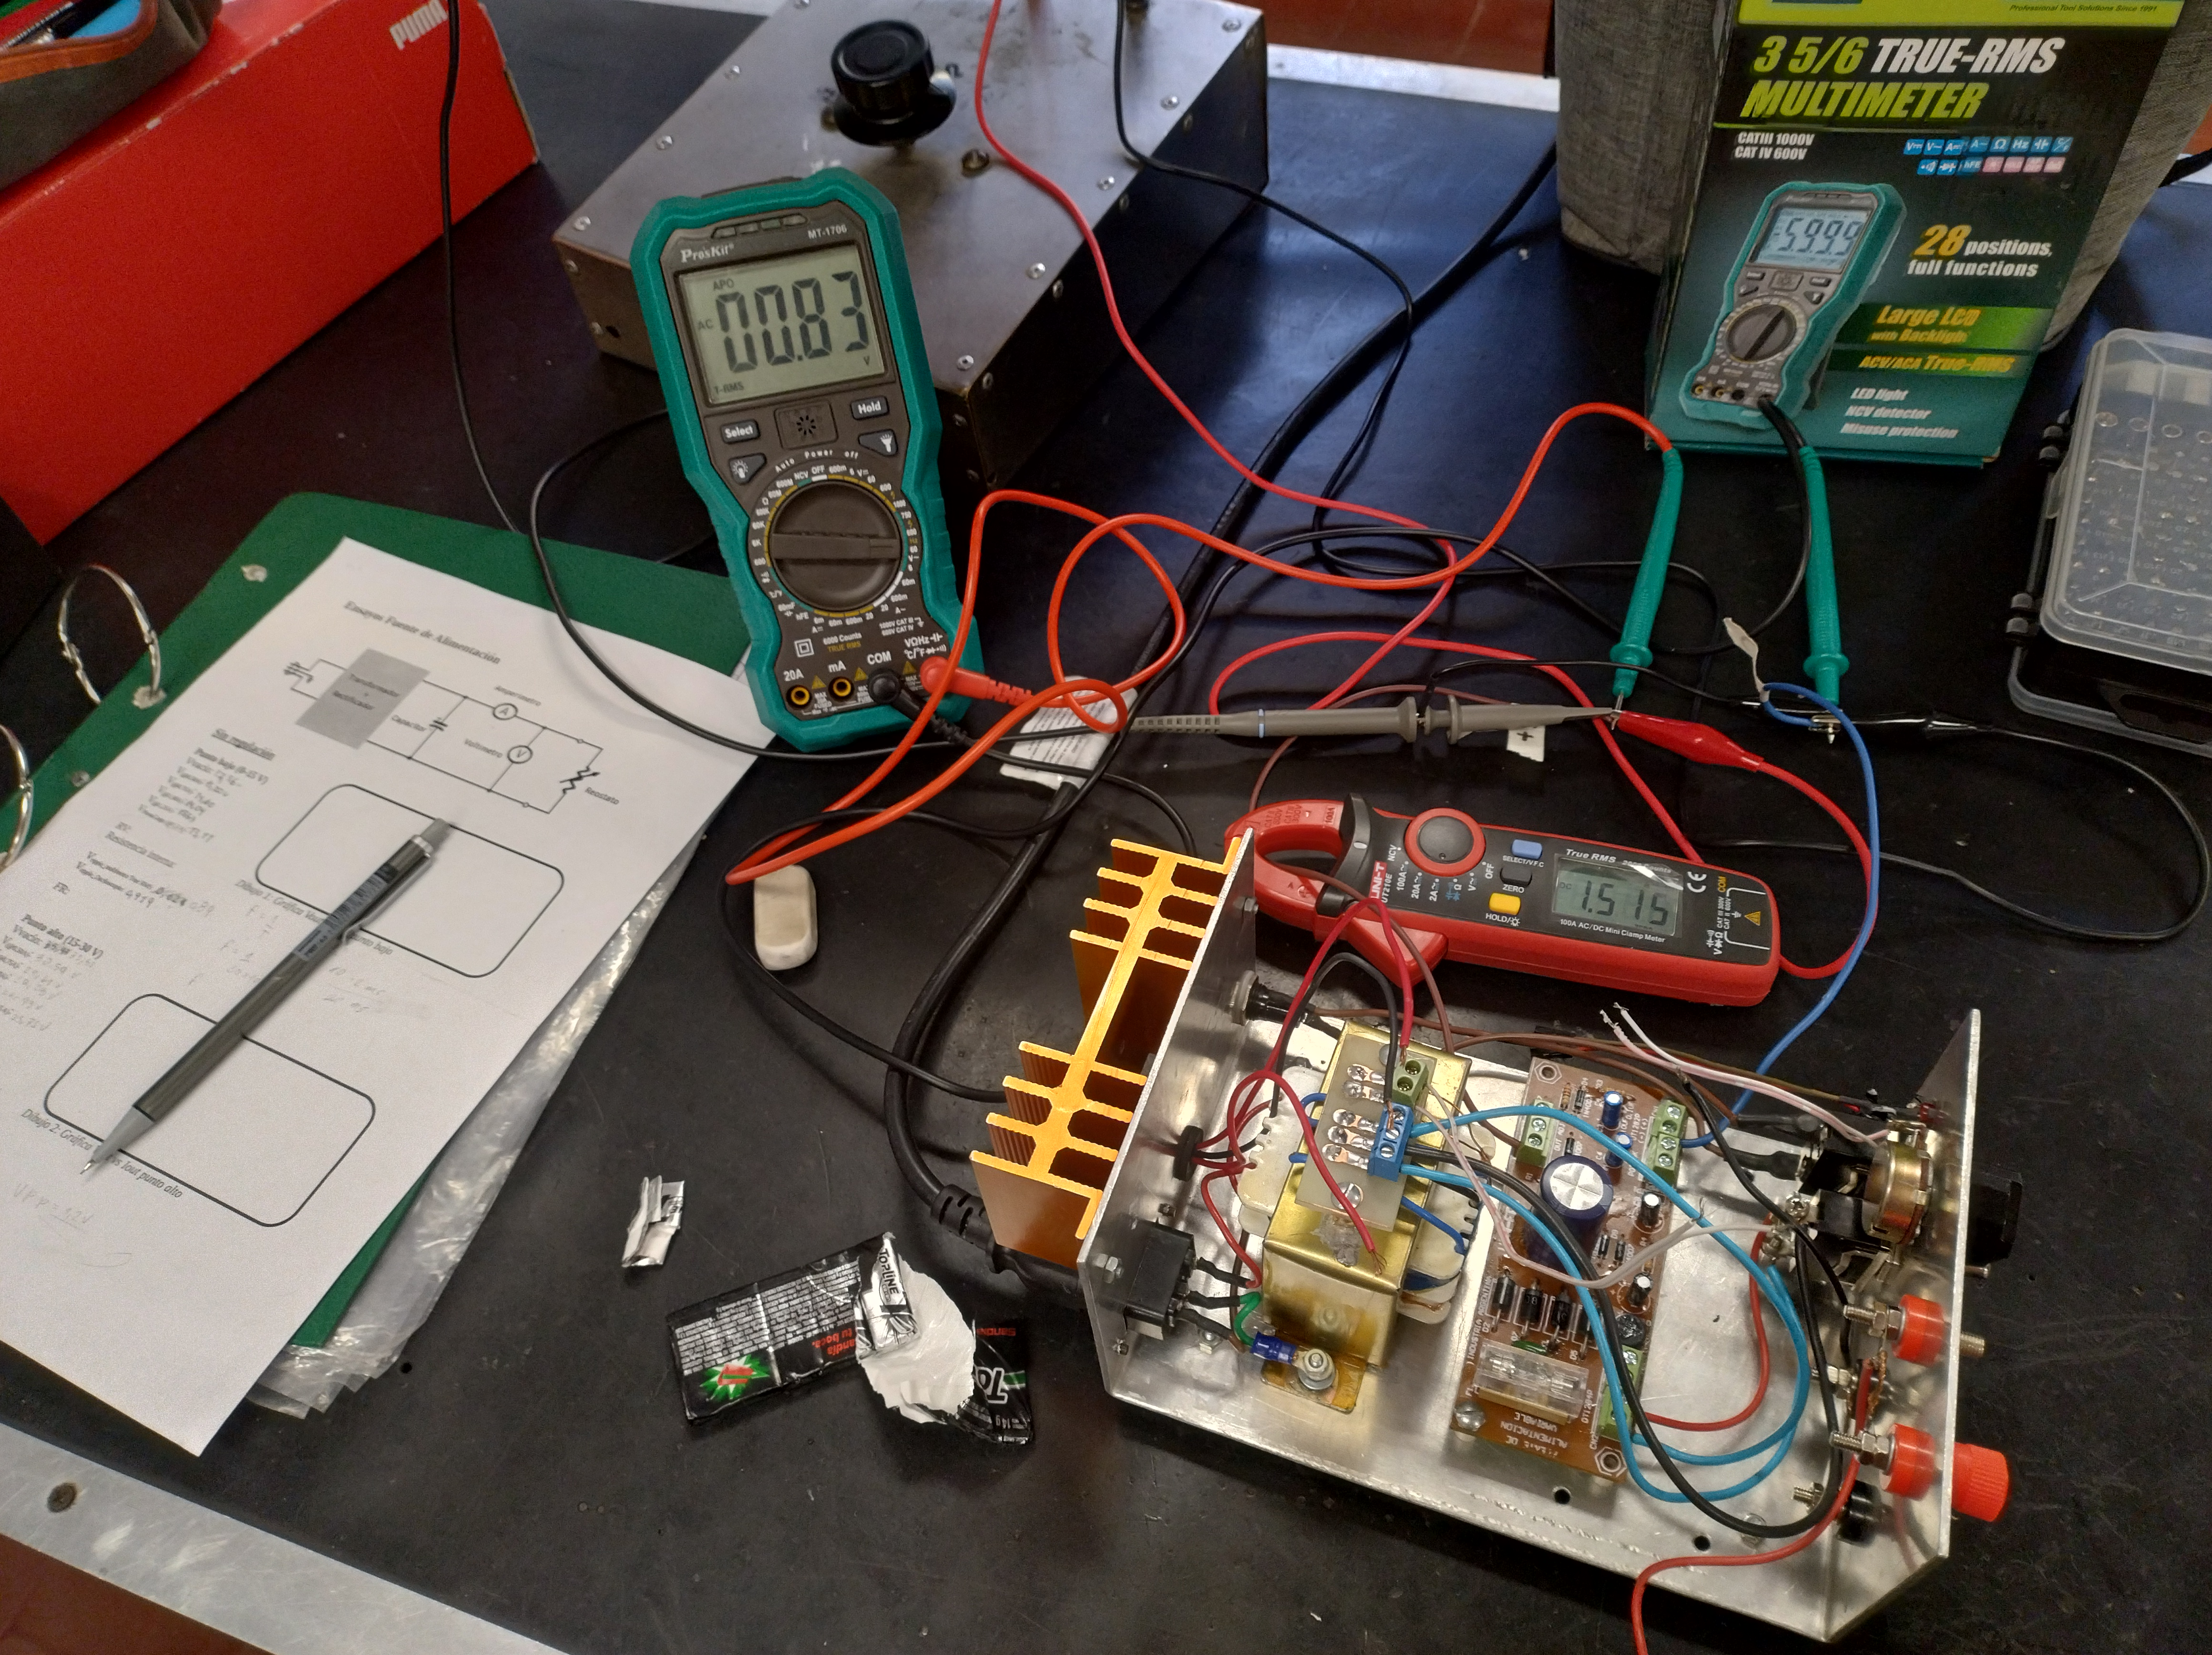
\includegraphics[width=0.9\linewidth]{./imagenes/riplle_alta_multimetro.jpg}
    \captionof{figure}{Medición de ripple en alta tensión (multímetro).}
\end{center}

\begin{center}
    \centering
    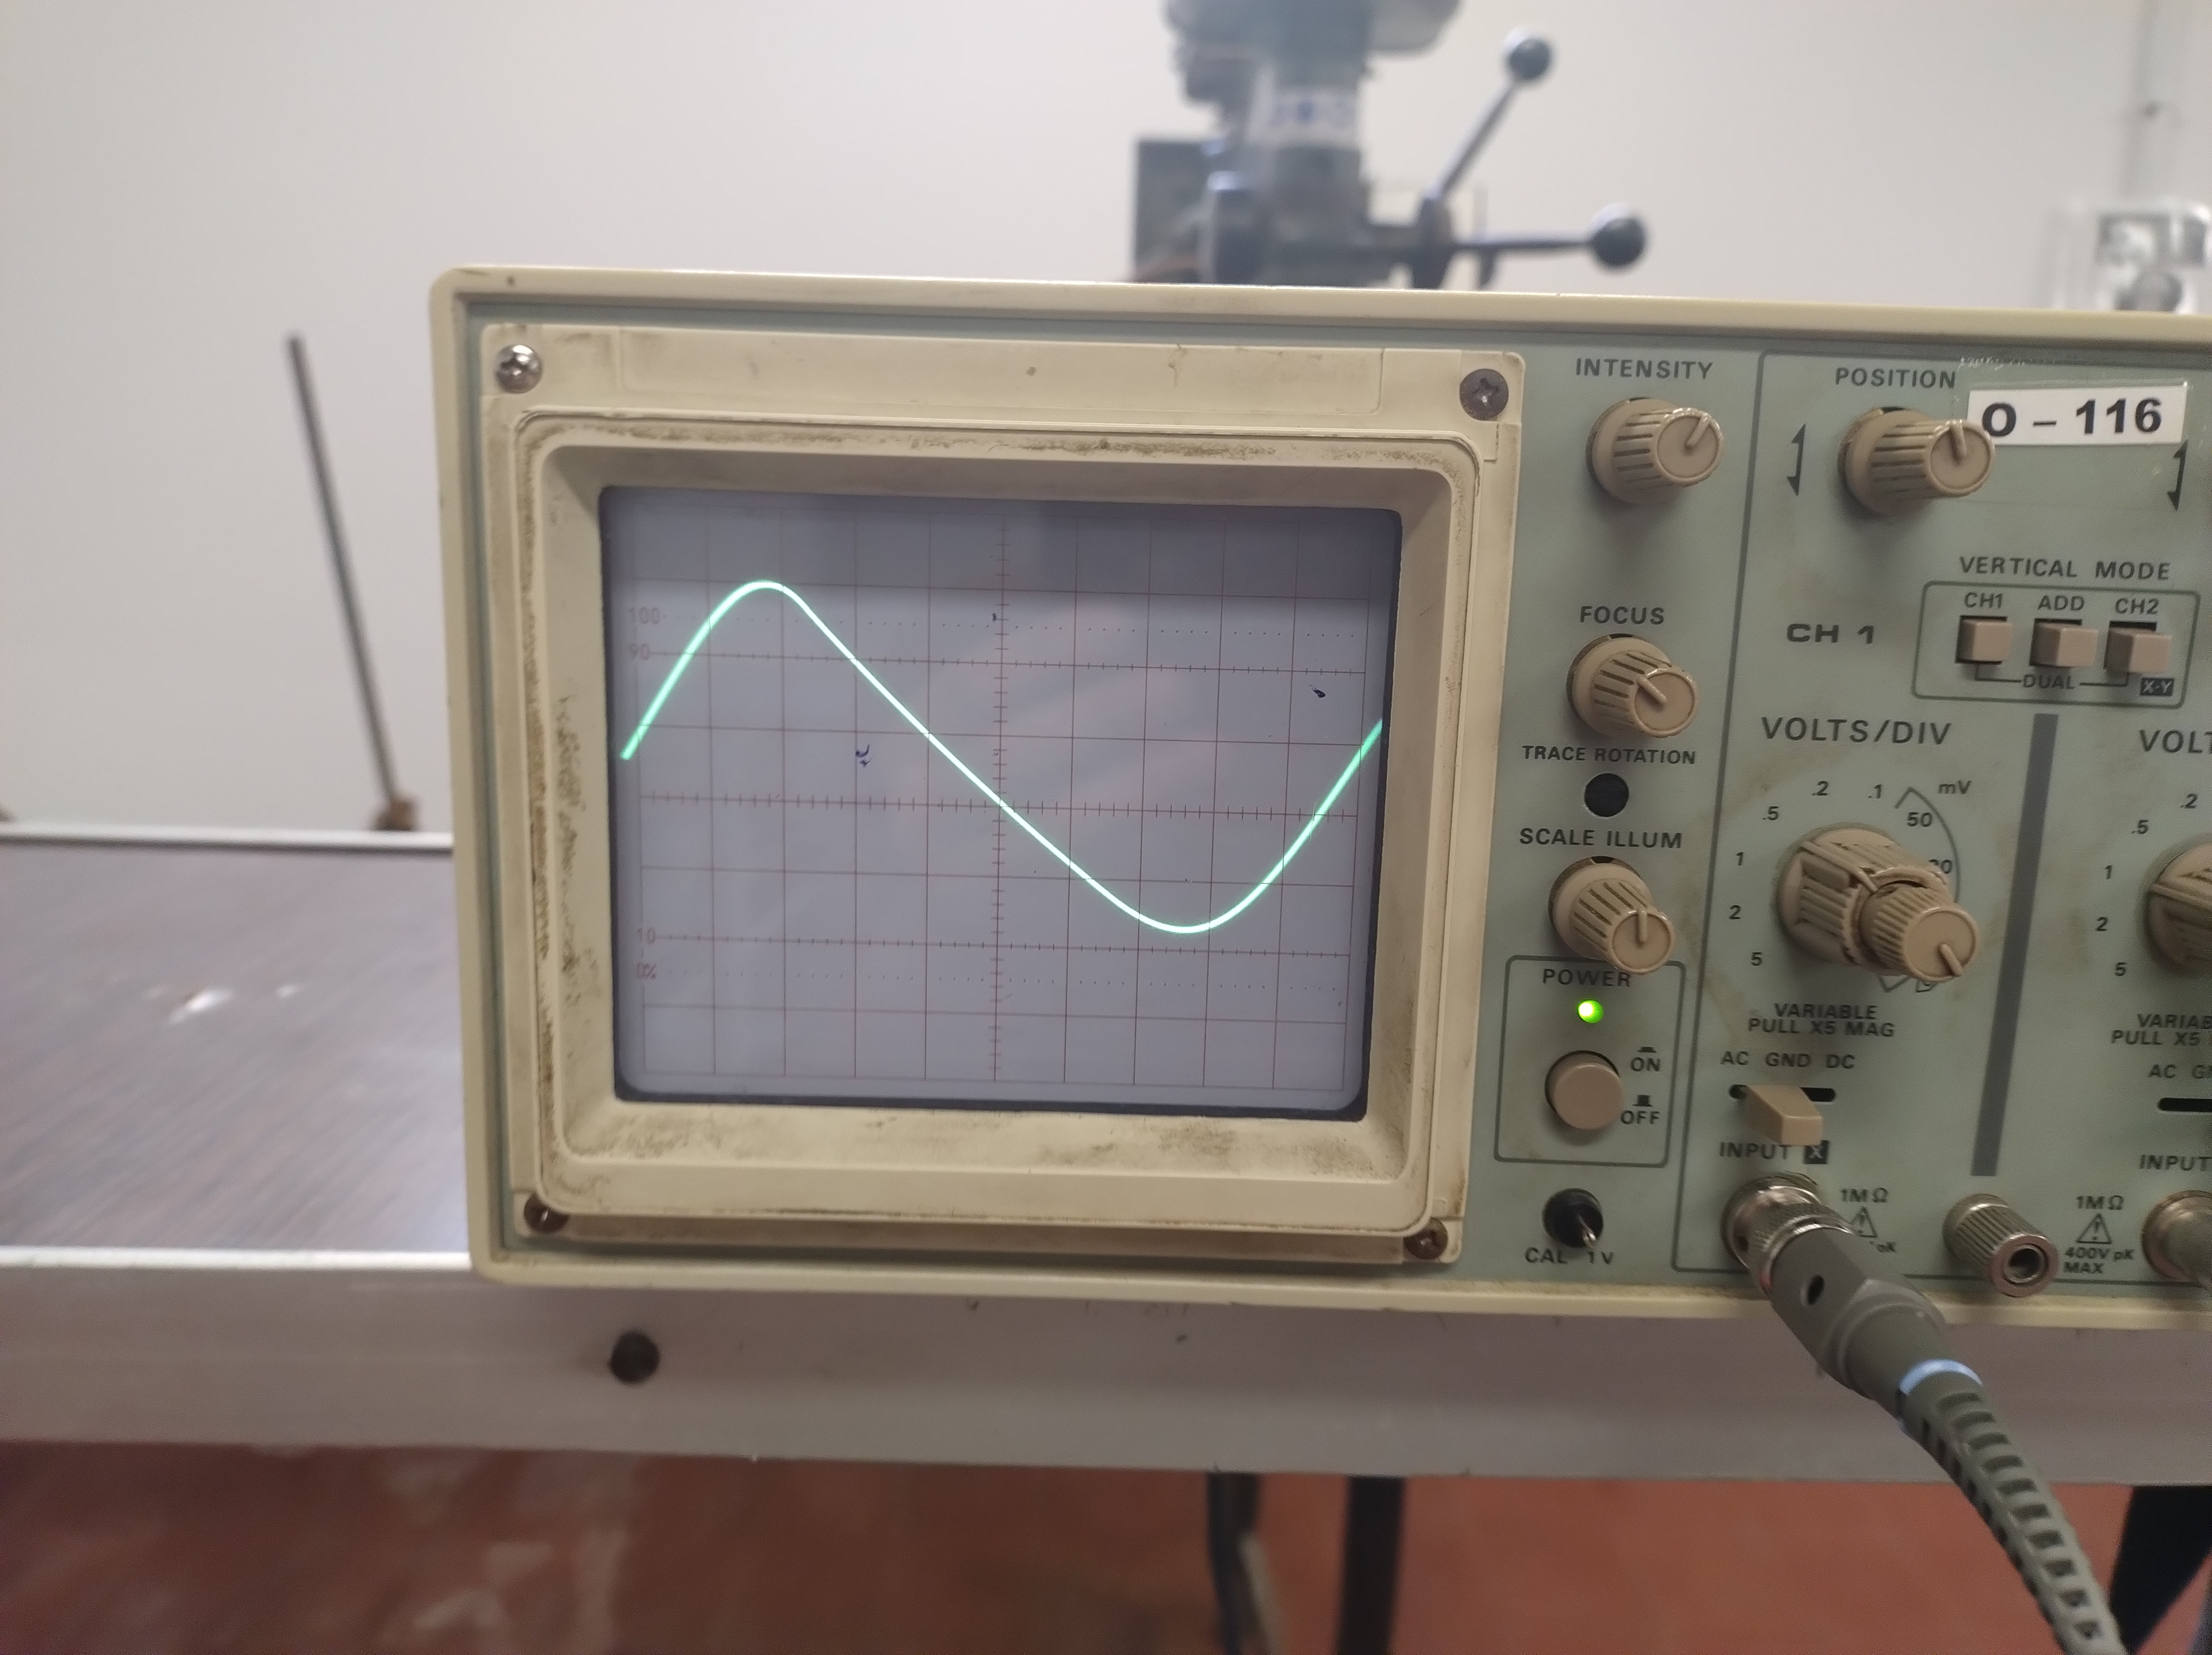
\includegraphics[width=0.9\linewidth]{./imagenes/riplle_alta_osc.jpg}
    \captionof{figure}{Medición de ripple en alta tensión (osciloscopio).}
\end{center}


\columnbreak{}
\text{}